\section{Introduction}

Mass spectrometry has evolved as a powerful tool for the high-throughput
analysis of complex protein mixtures, producing immense
amounts of data \cite[]{aebersold_mass_2003}. 
Dedicated software is essential for the identification of peptides and proteins
from tandem mass spectra (MS/MS).
Commercial programs for the evaluation of MS/MS data 
\cite[]{eng_approach_1994, perkins_probability-based_1999}
may represent a bottleneck because obtained licenses often apply to a 
certain maximum number of CPU cores and thereby limit the throughput of the 
data evaluation pipeline.
In addition to commercial software, a number of free and open source 
software tools for the evaluation of mass spectrometric data has been devised
\cite[]{geer_open_2004, craig_tandem:_2004}. 
As shown in a comparative study, these programs are able to compete with 
commercial software \cite[]{balgley_comparative_2007}.

The increasing variety of freely available tools for different purposes, 
including peptide and protein identification or quantitation, allows for 
manifold alterations in the choice of individual programs and their arrangement 
in an MS/MS data evaluation pipeline.
Most programs are controlled via the command-line interface (CLI), which is
necessary in order for the program to be included into an automated pipeline.
On the other hand, this mode of interaction makes the program less accessible 
to users.
Some programs are delivered with a dedicated graphical user interface (GUI)
which facilitates changing parameters and running the program. 
However, in order to create an automated processing pipeline in which multiple 
programs are chained together, CLI tools must be used and programming knowledge 
is required.

The Trans-Proteomic Pipeline (TPP, \cite[]{keller_uniform_2005}) aims to 
resolve some of the outlined issues by providing a web browser-based GUI to 
various programs and offering pre-defined workflows for various tasks. 
Although rich in functionality, TPP offers little workflow flexibility, as the 
user can either choose between executing single processing steps, or activate 
distinct processing steps in a pre-defined pipeline.
The addition of novel processing steps is non-trivial.

TPP requires the installation of an Apache web server which users can interact
with through a web interface.
In addition to the limited interaction capabilities of web-based user interfaces,
this setup also requires users to upload potentially large input files such as 
mass spectra or protein databases to the server.
Unfortunately, such a centralized approach does not take advantage of the 
massive processing power available in today's commodity computers.

Another alternative is the OpenMS Proteomics Pipeline (TOPP, 
\cite[]{kohlbacher_topp_2007}).
TOPP is built on top of the OpenMS C++ library, which provides mass 
spectrometry-related functionality. 
In comparison to TPP, TOPP offers decentralized data processing and provides a 
native GUI which does not require a web browser. 
The TOPP Pipeline Assistant (TOPPAS) allows for the visual construction of 
proteomic workflows and therefore greatly facilitates the construction of mass 
spectrometric data evaluation workflows.
However, the addition of novel tools is not possible without modifying and 
recompiling TOPPAS, a task which requires advanced programming skills.

\begin{figure}
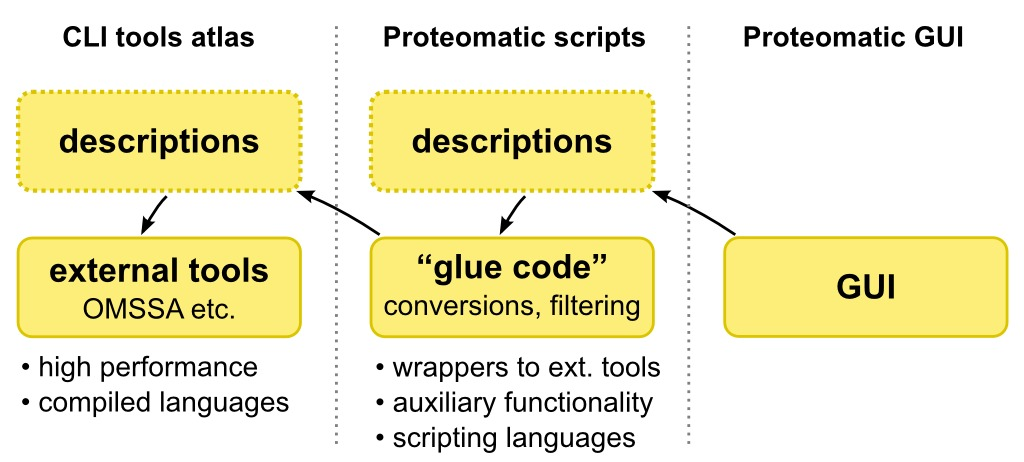
\includegraphics[width=0.48\textwidth]{craft/distinct-parts.jpg}
\caption{
    {\bf Separation of functionality from user interaction via descriptions.}
    Descriptions of external tools include the parameters of a program, its
    input and output files, and, if the software is freely available, download 
    locations for various operating systems.
    All descriptions are stored in a public repository existing independently of 
    the tools.
    Using the information from the repository, it is then possible to dynamically create
    a GUI to an external program, and, if possible, also download the software if it is not
    yet available on the user's computer.
    In addition, a distinction is made between high-performance tools and auxiliary
    processing steps. 
    Time-critical tools are usually implemented in compiler languages such as C or
    C++ to achieve high execution speed. 
    On the other hand, simple filtering or conversion steps may be implemented
    in scripting languages such as Ruby, Python, PHP or Perl, which generally
    offer more straightforward development and more compact source code.
}
\label{fig:distinct-parts}
\end{figure}

\begin{figure*}
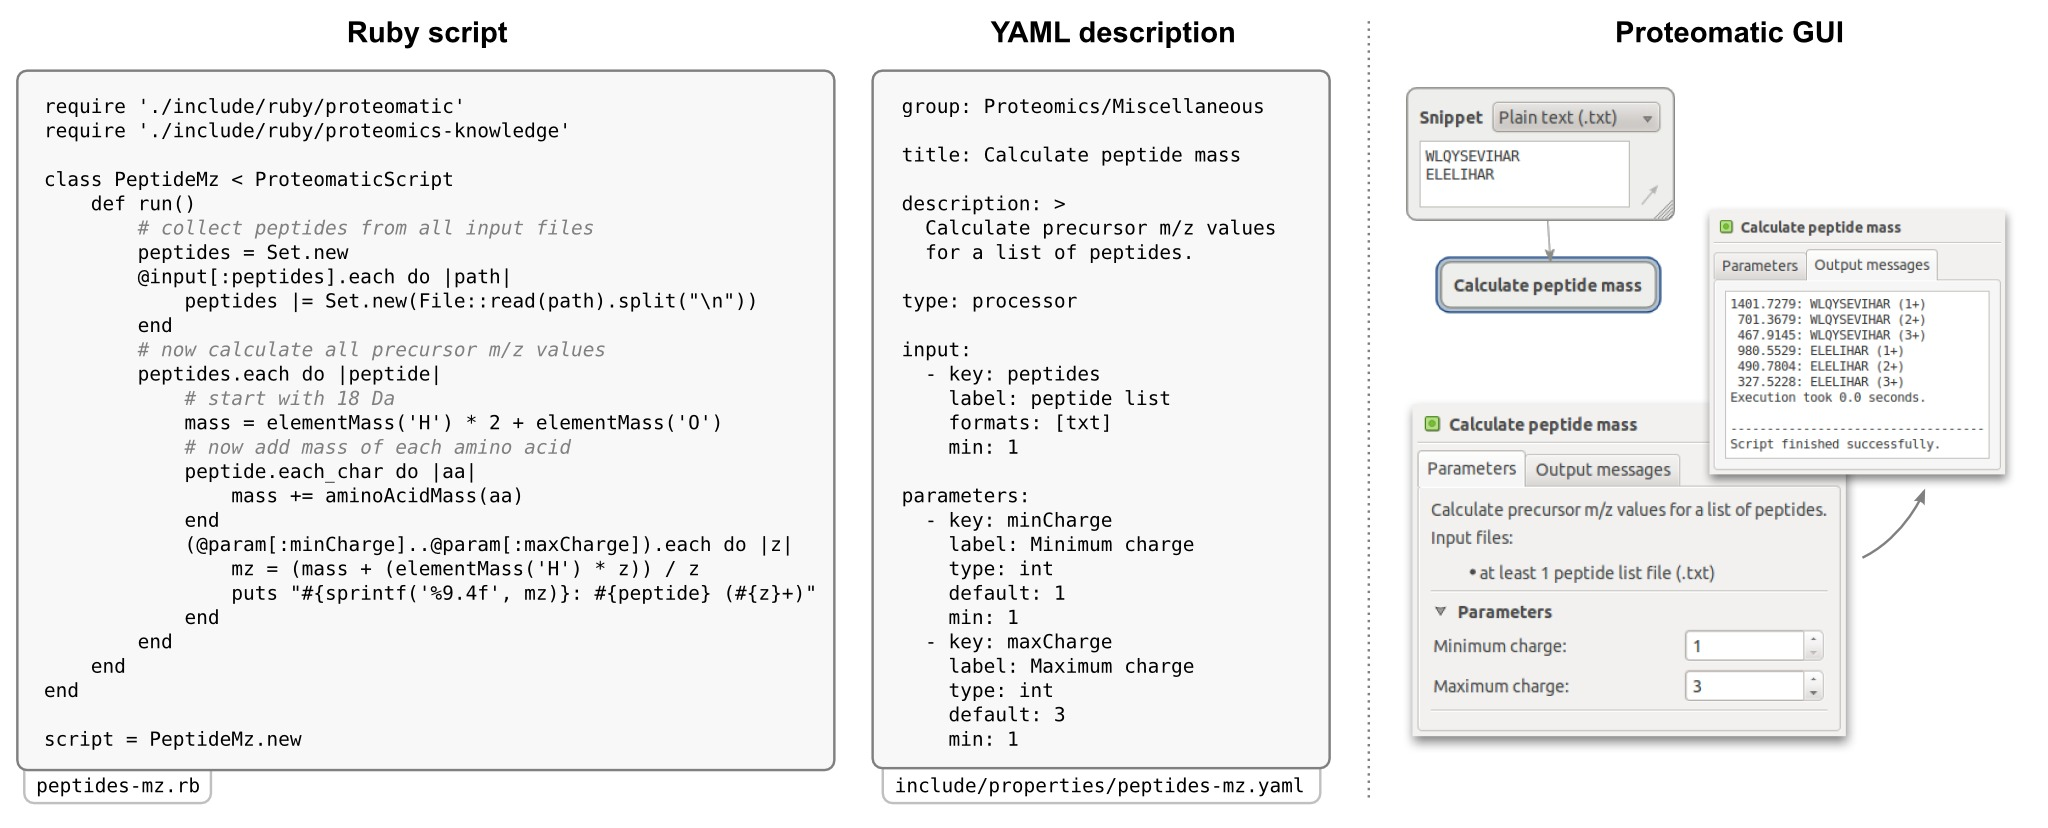
\includegraphics[width=\textwidth]{craft/example-script-2.jpg}
\caption{
    {\bf Example of a Proteomatic script for calculating precursor {\em m/z} 
    values.}
    The Ruby script implements the functionality. 
    Information about user-definable parameters (mininum and maximum precursor charge) 
    and the input files is stored in a separate, YAML-formatted 
    description file. 
    The connection between the two files is defined implicitly via their 
    filename.
    The Proteomatic GUI uses the description to construct widgets for 
    changing parameters and for integrating the script into a processing
    pipeline.
    In this example, a {\em text file snippet} is used to specify an input file
    in the GUI.
    To the script, this snippet appears as a regular input file.
    In order to facilitate future contributions, other scripting languages than 
    Ruby may be used to implement scripts.
}
\label{fig:example-script}
\end{figure*}

Proteomatic, the system presented in this study, extends the concept of a 
decentralized, user-friendly mass spectrometric data processing pipeline by 
implementing a strict separation of functionality (CLI tools) and presentation 
(the GUI).
Both aspects are inherently distinct and a separation allows for new external
programs to be added without modification of the GUI source code
(see Fig.~\ref{fig:distinct-parts}).
Proteomatic provides a GUI to external programs and auxiliary scripts which act
as ``glue code'' in between these programs.
External programs are used unmodified as provided by the respective authors,
and all three remaining aspects of the system (auxiliary scripts, descriptions, 
and the GUI) are stored independently in public Git repositories, thus 
facilitating future third-party contributions.
The fact that free software for various MS/MS data evaluation tasks is 
available allows for a decentralized mode of operation.
In such a setup, the user's computers are not only used to control a central 
server infrastructure, but are used to run the actual data evaluation software,
thereby increasing the overall throughput.
Therefore, in addition to decentralization, operating system independence is a 
key aspect of Proteomatic, accomodating for the different operating system 
preferences of individual users.
Proteomatic already provides a complete peptide and protein identification workflow
using OMSSA for protein database searching and a collection of auxiliary scripts
to provide false positive rate (FPR) estimation \cite[]{elias_target-decoy_2007}
and protein grouping to minimize the issue of ambiguous protein identifications
due to non-proteotypic peptides \cite[]{nesvizhskii_interpretation_2005}.

In addition to identification, peptide and protein quantitation via mass 
spectrometry has become an important aspect of mass spectrometric analysis 
\cite[]{kline_protein_2010, schulze_quantitation_2010}. 
Various programs for peptide and protein quantitation in metabolically labeled 
samples have been published \cite[]{han_quantitative_2001, li_automated_2003,
saito_ayums:_2007, park_quantitative_2008, cox_maxquant_2008, 
mortensen_msquant_2010}, with different platform support and label handling 
capabilities. 
In order to provide an operating system-independent peptide quantitation tool
for metabolically labeled samples, we introduce qTrace, which, like OMSSA, can be 
used within Proteomatic via an external program description.
qTrace searches for the isotope envelopes of previously identified sister 
peptides in MS1 full scans and allows for various labeling strategies, 
including stable isotopic labeling by amino acids in cell culture (SILAC) 
and \textsuperscript{15}N labeling.

\section{Concept}

From the user's perspective, Proteomatic provides a visual, interactive way to 
create and execute mass spectrometric data evaluation workflows.
Input files can be added to a canvas and connected to individual processing 
steps (e. g. {\em Run OMSSA}) which can be picked from a menu. 
Processing steps may provide output files which can in turn be connected to 
other processing steps, thus forming a directed acyclic graph that represents 
the processing pipeline in a visual way.
Whenever processing steps require external programs (such as OMSSA), these 
dependencies are resolved automatically using publicly available download 
locations, if possible.
Once the pipeline has been set up, it can be started at the click of a button.
% -----------------------------------------------------------------------------

On the conceptual level, albeit transparent to the user, Proteomatic is split into 
three distinct parts, as depicted in Fig.~\ref{fig:distinct-parts}:

\begin{enumerate}
\item program descriptions (CLI tools atlas)\footnote{http://github.com/specht/cli-tools-atlas}
\item Proteomatic scripts\footnote{http://github.com/specht/proteomatic-scripts}
\item Proteomatic GUI\footnote{http://github.com/specht/proteomatic}
\end{enumerate}

The separation of functionality from the GUI is achieved through the use of
the external program descriptions which provide all necessary information to
automatically construct a GUI for a certain external program and to allow
its incorporation into a pipeline.

\subsection{Support for multiple scripting languages}

The default scripting language for the Proteomatic scripts is Ruby.
However, we acknowledge the fact that several different scripting languages 
have been co-existing for some time.
In order to enable contributions from as many programmer communities as possible, 
Proteomatic provides an {\em any language hub}, which enables the use of the 
Proteomatic framework from scripting languages other than Ruby.

\subsection{File tracking}

To enable the reconstruction of individual processing steps, a feature 
called {\em file tracking} can be used while running a pipeline. 
When file tracking is enabled, a concise report is compiled upon successful 
completion of any script, containing information about all parameters, input
and output files, and the script's status messages. The report also 
contains MD5 checksums of all involved files to facilitate the identification 
of result files at a later time even if files have been moved or renamed.

\section{Implementation}

Each of the aforementioned three distinct parts of Proteomatic is implemented in 
a different context.

\subsection{CLI tools atlas}

The information about various free and commercial mass spectrometry-related 
programs is stored as YAML-formatted descriptions \cite[]{ben-kiki_yaml_2005}.
These descriptions contain information about the parameters and input/output 
files of a program and, in the case of free software, download locations for 
various platforms. 
Possible parameter types include integer and real numbers, strings, text 
fields, drop-down boxes, and boolean flags.
The storage of the CLI tools atlas in a publicly accessible Git repository
facilitates the incorporation of novel programs into a pipeline.

\begin{figure*}
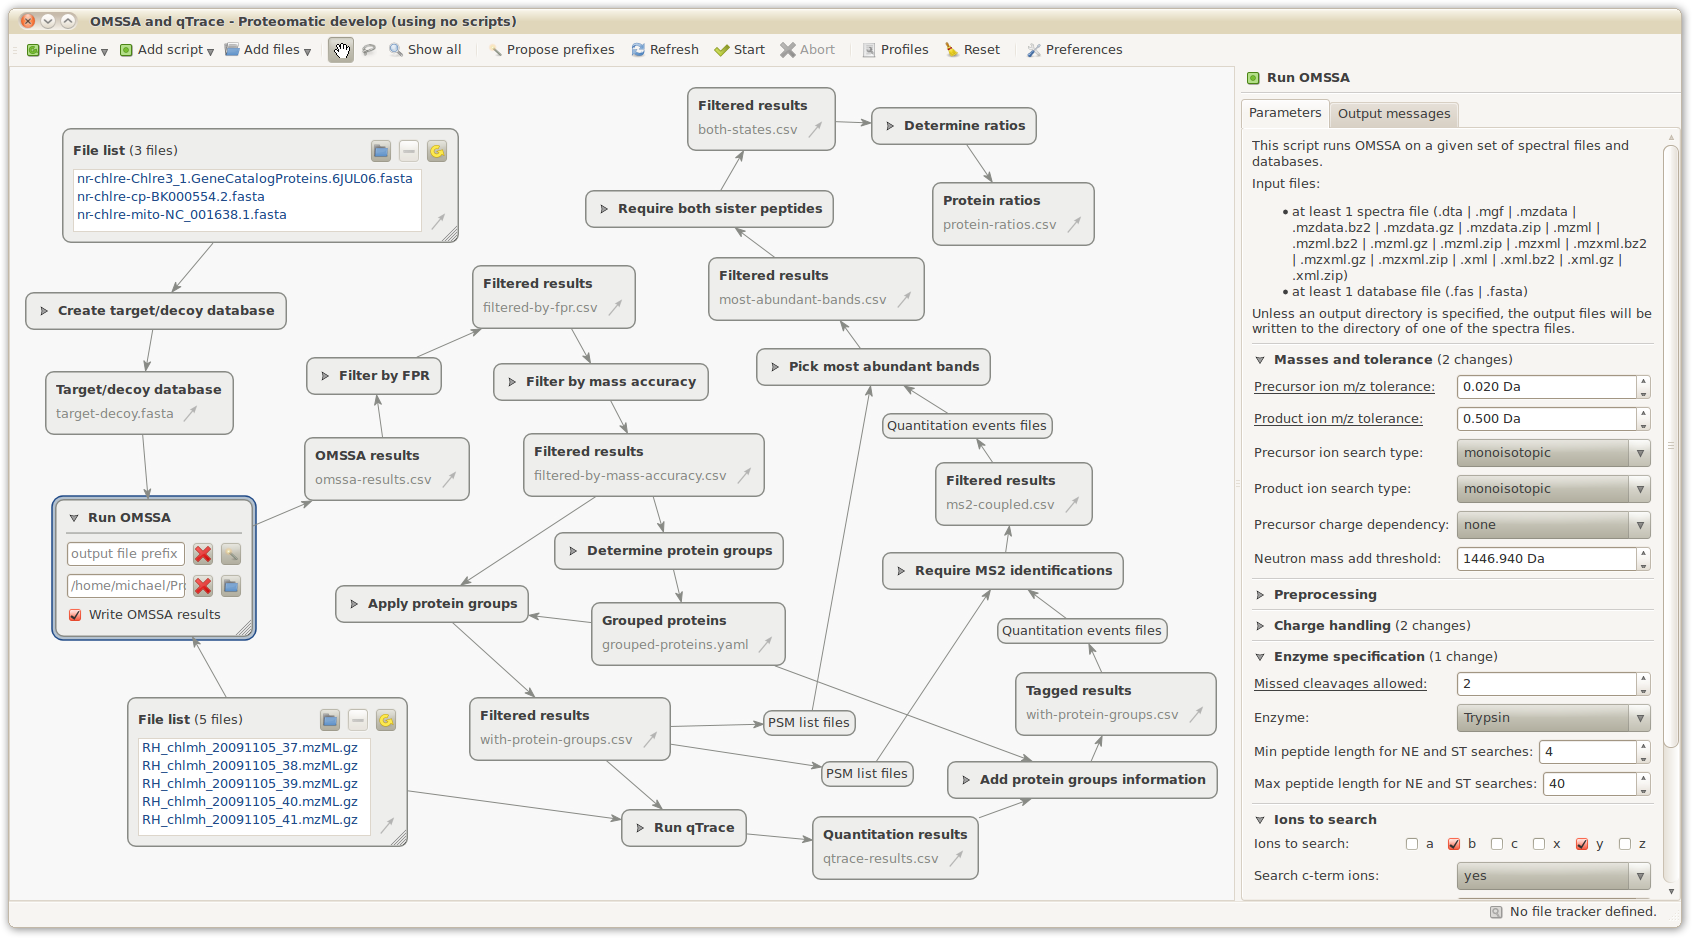
\includegraphics[width=\textwidth]{proteomatic-new-figure.jpg}
\caption{
    {\bf Proteomatic screenshot demonstrating a proteomics pipeline for
    protein identification and quantitation.}
    This Proteomatic screenshot demonstrates an example pipeline for protein 
    identification and quantitation, using a target/decoy approach in 
    conjunction with OMSSA for protein identification and qTrace for protein 
    quantitation. 
    The processing pipeline can be seen on the left hand side of the window, 
    composed of existing input files (blue font), yet to be created output 
    files (gray font) and scripts in between. The right hand side of the window 
    contains the user-adjustable parameters of the {\em Run OMSSA} script 
    (see also Supplementary Figure S1).
    Once a pipeline has been constructed, it can saved and reused at a later
    time.
}
\label{fig:pipeline}
\end{figure*}

\subsection{Proteomatic scripts}

The Proteomatic scripts implement all functionality available in Proteomatic.
Features such as automatic software downloading and file tracking are provided
by a framework implemented in Ruby.
Scripts implemented in other languages access the same functionality through
the any language hub.

As available for external programs, a YAML-formatted description also exists for 
every Proteomatic script. 
If a script acts as a wrapper around an external program, its description may 
reflect the external program's parameters by including its description from 
the CLI tools atlas.

Any Proteomatic script must subclass the {\tt ProteomaticScript} class and 
implement the {\tt run()} method, in which three instance variables {\tt input}, 
{\tt output}, and {\tt param} have been made available by the underlying 
framework (see Fig.~\ref{fig:example-script}).
These variables reflect the information stored in the YAML description and the 
user's choice of parameters and input/output files. 
After the class has been defined, an instance of this class is created, 
thereby implicitly calling the superclass constructor which sets up all
necessary variables.
Required external programs are downloaded and unpacked.
Finally, if legal parameter values have been specified, the {\tt run()} method
is called.
While currently, the script is run immediately from the superclass 
constructor, this setup would also allow for enqueueing and executing the script
on a remote system.
This would facilitate a hybrid centralized/decentralized system in which 
pipelines can be built locally but the execution of a pipeline may be delegated 
to a dedicated machine, keeping the user's computer responsive.

The {\tt ProteomaticScript} class automatically handles a number of command line 
switches common to all Proteomatic scripts:
The {\tt --help} switch prints a human-readable help message derived from
the YAML-formatted description of the script. 
The {\tt ---yamlInfo} switch provides the same information in a computer-readable 
fashion but may also indicate that external programs required by the script are
not available on the computer yet.
In the case of free software, unresolved dependencies may be resolved by specifying 
the {\tt --resolveDependencies} switch.

\subsection{Proteomatic GUI}

The Proteomatic GUI is implemented as a C++/Qt application, enabling seamless 
integration with Windows, Mac OS X, or Linux desktops.
The application does not provide any MS/MS data evaluation functionality but
acts as a user interface layer on top of the Proteomatic scripts.

Users may choose individual processing steps (implemented as scripts) from a 
menu (see Fig.~\ref{fig:pipeline}). 
Every script is depicted as a box on a canvas, and parameters of
the currently selected script can be modified in the right-hand pane
of the window.
Files can be added to the canvas and specified as input files to a script by 
connecting both boxes via an arrow.
By connecting the output files of one script to another script, increasingly
complex pipelines can be constructed.

Additionally, an equivalent of the {\em for loop} available in many programming 
languages can be expressed by turning a {\em file list} into a {\em file batch}. 
In this mode, a script is called once for every input file in the batch, 
thus creating one output file for every input file, as opposed to file lists,
where a single output file is created for all input files.
It is also possible to specify multiple input batches, if corresponding files 
can be determined unambiguously.

\begin{figure*}
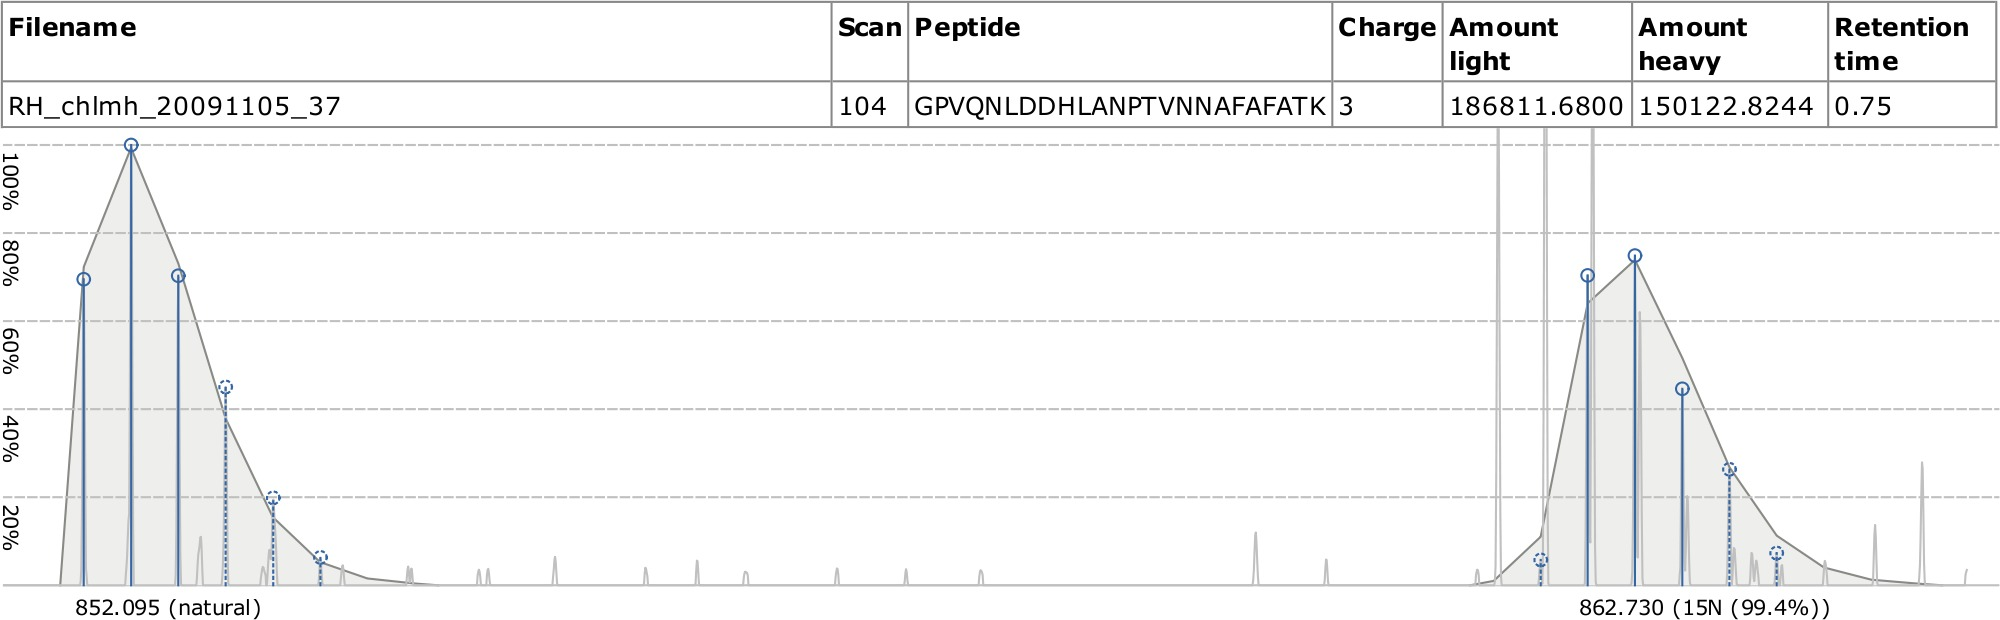
\includegraphics[width=\textwidth]{qtrace-figure.jpg}
\caption{
    {\bf An example sister peptide pair from a 
    \textsuperscript{14}N/\textsuperscript{15}N labeled 
    {\em C. reinhardtii} sample as observed in a MS1 full scan. }
    {\em Required} peaks with a relative peak intensity of at least 50\% are 
    denoted by solid circled lines, {\em considered} peaks with a relative peak 
    intensity of at least 1\% are denoted by dashed circled lines. 
    The areas shaded in gray depict the theoretical isotope envelopes fitted to
    the observed {\em required} and {\em considerded} peaks and yield a light/heavy
    ratio of 1.24 for this scan.}
\label{fig:qtrace}
\end{figure*}

\section{Peptide and protein quantitation with qTrace}

In order to provide a tool for the quantitation of metabolically labeled 
peptides and proteins, we propose qTrace, a novel operating system-independent 
quantitation program. 
qTrace uses a list of peptides which have been previously identified via MS/MS
(`target peptides') and performs peptide quantitation based on the corresponding 
precursor ions in full scans.
Users may choose from a list of predefined labels or manually specify a 
labeling strategy using a syntax which accurately describes the label applied 
to the sample.
Labels can be defined by specifying certain isotopes such as `15N' or `13C'.
Combinations of multiple isotopes are possible. 
Isotopes may be followed by a labeling efficiency: `15N (0.994)'
indicates that 99.4\% of all nitrogen atoms in the labeled sample are 
\textsuperscript{15}N isotopes, and the remaining 0.06\% are 
\textsuperscript{14}N isotopes. 
Isotopes, or combinations thereof, may be prefixed with an 
amino acid scope that constrains isotopes to certain amino acids: 
`R 13C' indicates \textsuperscript{13}C atoms in all arginine residues (like for 
isotopes, multiple amino acids may be specified). 
To accommodate for the effect that labeled arginine residues may lead 
to labeled proline residues due to their shared amino acid biosynthesis pathways, 
variable labels may be defined by suffixing an amino acid with the star 
symbol: `RP* 13C' indicates heavy carbon atoms in all arginine residues 
and also variably in all proline residues, leading to $n$ additional labeled 
isotope envelopes, where $n$ is the number of proline residues.
Finally, an amino acid scope may be negated by using the caret symbol: 
`$\caret$R 15N' indicates \textsuperscript{15}N isotopes in all residues 
except arginine.

\subsection{Abundance estimation}

qTrace offers two modes of abundance estimation: (a) a {\em fixed peak count} 
mode and (b) an {\em isotope envelope fitting} mode. 

In the {\em fixed peak count} mode, a fixed number of required isotope peaks $n$,
including the monoisotopic peak, is defined by the user.
qTrace calculates the {\em m/z} values of the respective isotope peaks 
\mbox{$A+0$} to $A+(n-1)$ for every unlabeled and labeled target peptide within 
a user-definable charge state range and stores these target peaks as 
`required present'. 
In addition, the $A-1$ peak of the light sister peptide is stored as 
`required absent', because its presence for one peptide would imply 
that its alleged $A+0$ peak might in fact be the $A+i$ peak of 
another peptide. 
The calculated {\em m/z} values are then matched to the observed {\em m/z} 
values within a user-defined precursor mass tolerance.
Whenever all presence and absence requirements are met for a certain unlabeled 
or labeled peptide, its abundance is estimated by summing the peak heights of 
all peaks stored as `required present'. 

Using the {\em isotope envelope fitting} mode, peak intensities are calculated in 
addition to the {\em m/z} values by predicting the shape of the 
isotope envelope from the elemental composition of every target peptide. 
Instead of defining a fixed number of isotope peaks per precursor ion, `required
present' peaks are defined using a relative intensity threshold in respect to the
highest peak of the predicted isotope envelope.
This leads to a variable `required isotope peak' count per peptide, depending on 
its elemental composition.
Typically, a relative intensity threshold of 50\% is used to define `required 
present' peaks. 

All `required present' peaks have to be present in the spectrum for the peptide 
to be identified.
In addition, a variable number of `considered if present' peaks may be defined
via a second threshold (typically 1\%). 
All `required present' and `considered if present' {\em m/z} values are matched 
to the observed {\em m/z} values.
If all required peaks are present in the scan, the union of all `required' and
`considered' peaks is fitted to the theoretical isotope envelope, taking peak
heights into account.
A fitting error is determined and used to discard false matches.
Because the shape of the theoretical isotope envelope is taken into account, 
it is not necessary to check for the absence of the unlabeled $A-1$ peak.
The area under the fitted isotope envelope is then used as an estimate for
peptide abundance (see Fig.~\ref{fig:qtrace} and Supplementary notes).

\subsection{Result compilation}

For demonstration purposes, we assume the following experimental context:
\textsuperscript{14}N/\textsuperscript{15}N differentially labeled proteins from 
the unicellular green alga {\em Chlamydomonas reinhardtii} were mixed at equal 
protein concentration and fractionated by SDS-PAGE. After separation, protein 
bands were excised, digested with trypsin and analyzed by liquid chromatography 
coupled mass spectrometry.
Data evaluation of the resulting full and fragmentation scans was conducted via 
Proteomatic using OMSSA for identification and qTrace for quantitation. 

The output of qTrace is a list of peptide quantitation events in full scans.
Every quantitation event denotes unlabeled and labeled abundances of a peptide 
in a defined context (e.g. certain SDS-PAGE band and/or retention time),
at a certain charge state.
We call the combination of peptide, band, and charge the {\em PBC combination}
of a certain quantitation event.
Ratios are determined by dividing the sums of all unlabeled and labeled peptide
abundances within a PBC combination to accomodate for small retention time
shifts of sister peptides.
In addition, different PBC combinations can be regarded as independent observations 
of the peptide over retention time and a minimal PBC combination count can therefore 
be used as a filter criterion in a subsequent processing step.

The following filtering steps are provided by Proteomatic (see Figs.~\ref{fig:pipeline}
and \ref{fig:exp-setup}):

{\bf Add protein information.}
For every peptide quantitation event, the corresponding protein (or
protein group) is determined, and all quantitation events of peptides 
appearing in multiple proteins (or protein groups) are discarded.

\begin{figure*}
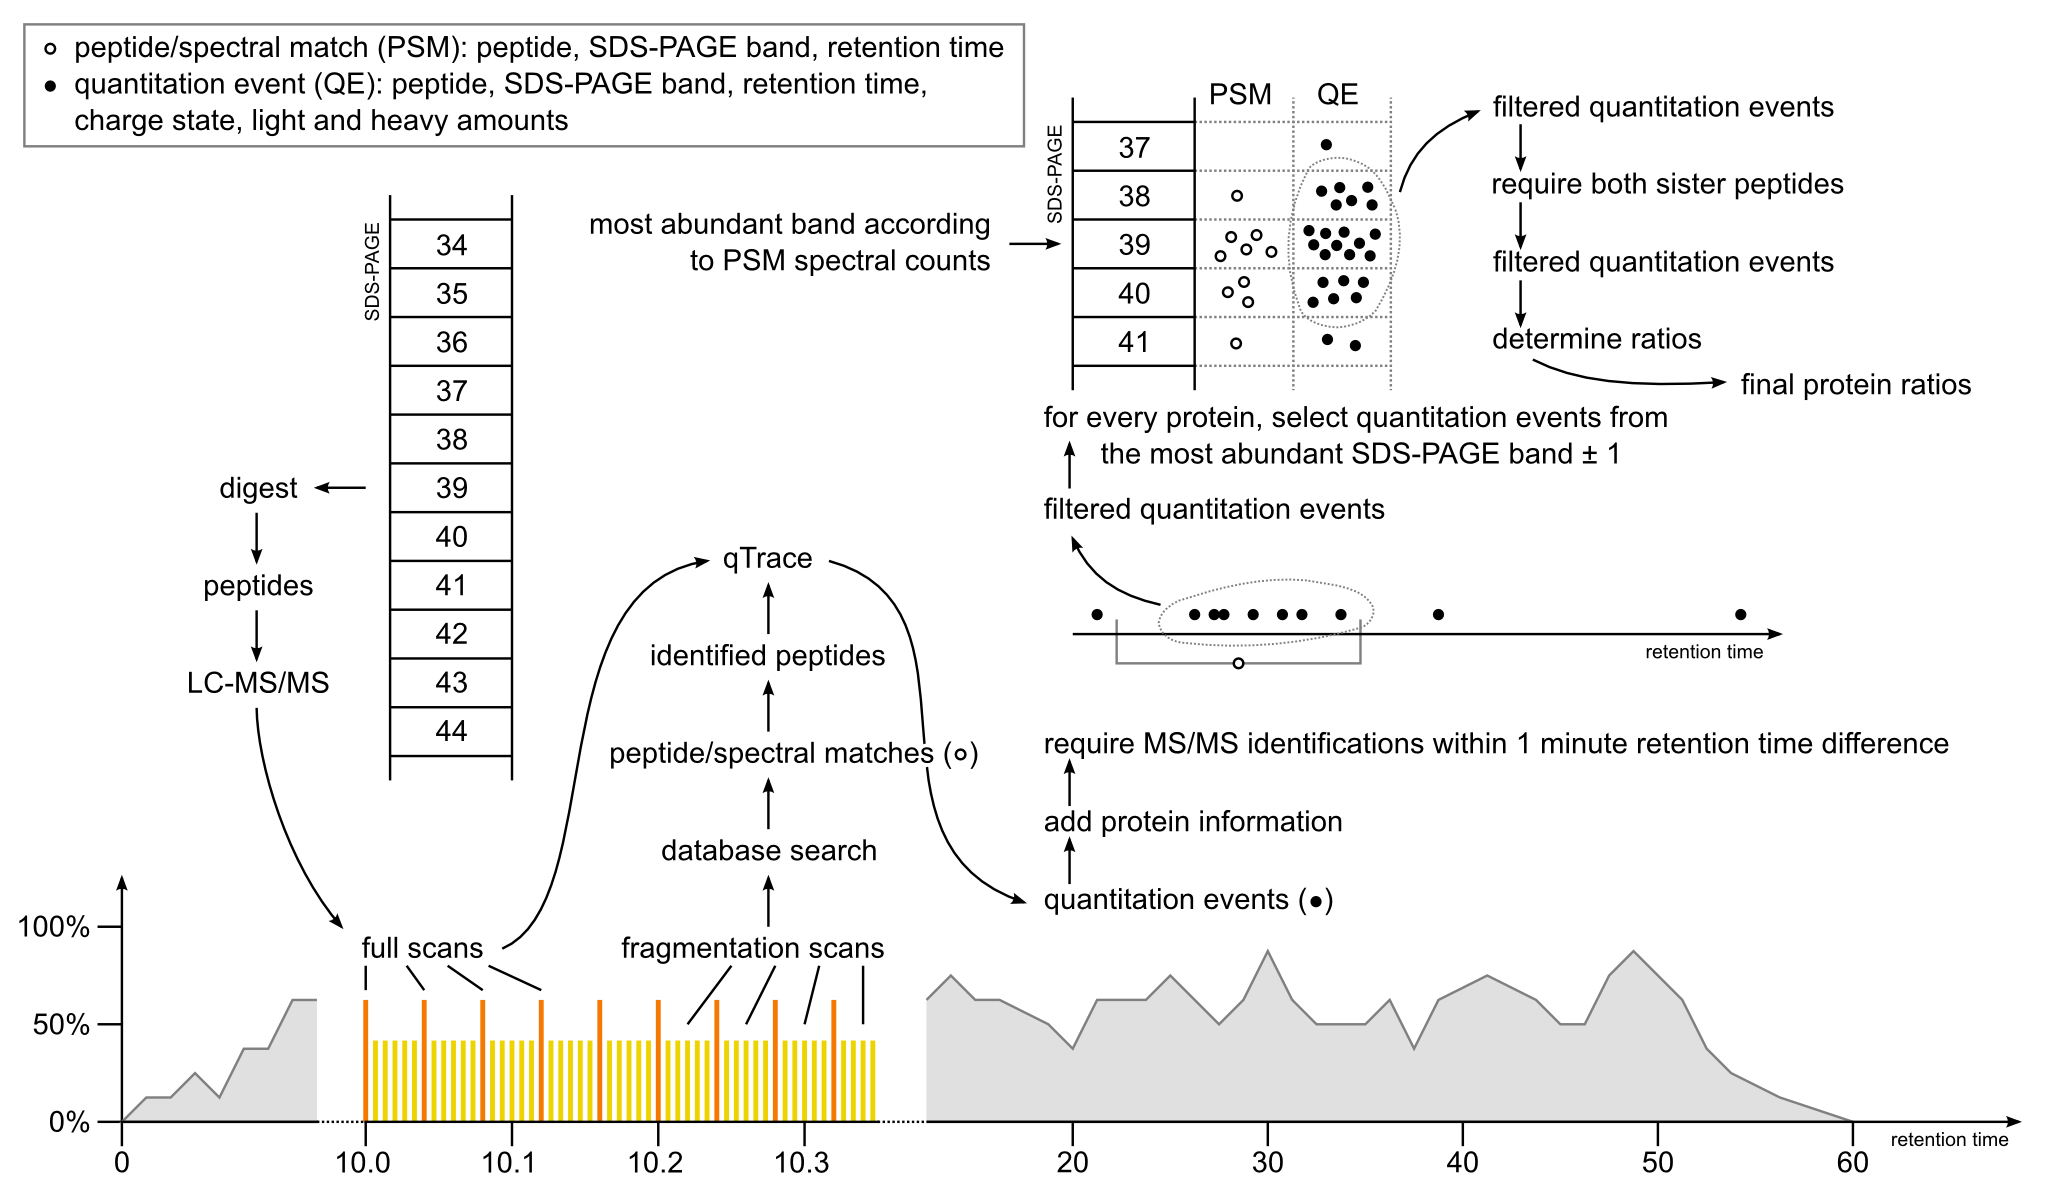
\includegraphics[width=\textwidth]{exp-setup.jpg}
\caption{
    {\bf Depiction of the experimental workflow for protein identification and 
    quantitation. }
    Protein samples are subjected to two steps of separation: (a) SDS-PAGE, in 
    which each sample is fractionated into distinct bands, and (b) HPLC, which 
    separates the digested peptides from each SDS-PAGE band according to their 
    hydrophobicity. 
    The peptides eluting from the HPLC are measured using the {\em Big 5} 
    method which produces full scans and fragmentation scans in an interleaved 
    pattern. 
    While the fragmentation scans are used to identify peptides via a database 
    search (e. g. using OMSSA), the full scans are used by qTrace to quantify 
    the previously identified peptides using their light and heavy precursor 
    masses.
    The resulting quantitation events (QE) are then filtered in such a way
    that MS/MS identifications are required within a short retention time 
    difference. 
    The peptide quantitation events are compiled to protein quantitation events
    by determining which protein a peptide belongs to and discarding all events
    from ambiguous peptides.
    In addition, the spectral counts derived from the MS/MS identifications are 
    used to determine the SDS-PAGE band in which a protein has been must 
    abundantly identified in, and only quantitation events from this band 
    ($\pm$1) are accepted.
    Finally, the protein ratios are determined.
}
\label{fig:exp-setup}
\end{figure*}

{\bf Require MS/MS identifications.}
All quantitation events for which no MS/MS identification exists in the same 
SDS-PAGE band within a user-defined retention time difference (1 minute by 
default) are discarded. This filter corresponds to the separation of the 
tryptic peptides via liquid chromatography.

{\bf Pick most abundant SDS-PAGE band.}
For every protein, the SDS-PAGE band in which the protein has been identified 
in most abundantly is determined, and only quantitation events stemming from 
this band ($\pm$ a user-defined tolerance, typically 1) are discarded. This 
filter corresponds to the fractionation step via SDS-PAGE.

{\bf Require both sister peptides.}
Quantitation events in which only one of the sister peptides (labeled or 
unlabeled) could be quantified can be considered less reliable than quantitation 
events in which both sister peptides could be quantified.
This is because the missing peptide might have escaped detection due to a 
post-translation modification resulting in a different precursor mass. 
This filter rejects all quantitation events in which one sister peptide has 
been quantified with an abundance of zero.

{\bf Determine ratios.}
In all previous processing steps, only abundances have been determined and 
filtered. 
This step determines actual ratios by dividing the sums of unlabeled and 
labeled abundances within every PBC combination and then determining the final 
protein ratio as the mean (and standard deviation) of the individual PBC 
combination ratios.
A high number of PBC combination ratios is favorable because every PBC 
combination may be regarded as an independent observation of a sister peptide 
pair.

\section{Results and discussion}

The pipeline depicted in Fig.~\ref{fig:pipeline} implements a complete 
protein identification and quantitation workflow, using OMSSA and the novel 
protein quantitation tool qTrace. 
In addition to these two programs, a number of auxiliary processing steps are
included to enable protein identification at a user-defined FPR using a 
target-decoy approach.
In addition, protein groups are automatically determined, increasing the yield of 
unambiguous peptides by grouping protein isoforms.

It should be noted that the flexibility of the pipeline allows for alterations 
in the data evaluation and that individual processing steps can be rearranged 
and new steps can be added with little effort in order to meet the requirements 
of the system at hand.

Proteomatic and qTrace have already been used in a recent study 
\cite[]{terashima_characterizing_2010} to characterize the anaerobic 
response of {\em Chlamydomonas reinhardtii}, yielding protein ratios for more
than 400 proteins using \textsuperscript{13}C-Arg labeled SILAC samples. 
A demonstration of qTrace handling \textsuperscript{14}N/\textsuperscript{15}N 
metabolic labeled samples can be found in Supplementary Figure S2.

In order to assess the performance of qTrace, we have conducted a comparison 
between the established protein quantitation program 
MaxQuant \cite[]{cox_maxquant_2008} and qTrace, which shows that qTrace performs 
comparably to MaxQuant, yielding similar ratios for 80\% of all identified 
proteins (Supplementary Figure S3).

\section{Conclusion}

Proteomatic provides a high-throughput data evaluation platform for protein
identification and quantitation, using a variety of freely available programs
downloaded automatically when required, thus providing a
straightforward system to evaluate large MS/MS data sets.

Through the use of scripting languages, existing functionality can easily be
adjusted and new functionality can be added using Ruby, Python, PHP, and
potentially any other operating system-independent scripting language.

The complete separation of functionality and presentation makes it possible to 
use Proteomatic from the CLI while still taking advantage of features such as 
file tracking and automatic downloading of required software.

We hope that the possibility to implement new processing steps in various 
scripting languages and the straightforward deployment to Proteomatic 
encourages community contributions and fuels the development of novel MS/MS 
data evaluation tools.

Proteomatic runs on Windows, Mac OS X and Linux, and is freely 
available at http://www.proteomatic.org.
